\section{DMR Simplex Betrieb} \label{sec:simplex}
Die einfachste Form eines DMR QSOs\footnote{Für alle nicht-Funkamateure: QSO ist eine Abkürzung die eine Verbindung zwischen zwei Amateurfunkstationen beschreibt, gelesen als \emph{Verbindung} oder \emph{Gespräch}.} ist der \aref{Simplexbetrieb}. Dabei wird eine direkte Verbindung zwischen zwei DMR Funkgeräten aufgebaut, die sich beide direkt erreichen können. Wie bei dem DMR Repeaterbetrieb, kann so eine Verbindung ein Direktruf, Gruppenruf oder auch ein sog. \adef{All Call} sein. 

\begin{figure}[!ht]
 \centering
 \documentclass{standalone}
\usepackage{tikz}
\usetikzlibrary{shapes.geometric}
\newcommand{\repeater}[3]{%
 \node ({#1}) at ({#2}) {%
  \begin{tikzpicture}%
   \draw [black,thick] (-.25,0) -- (0,0.5) -- (0.25,0) -- (-0.25,0);%
   \draw [black,thick,domain=-45:225] plot ({0.2*cos(\x)}, {0.5+0.2*sin(\x)});%
   \draw [black,thick,domain=-45:225] plot ({0.4*cos(\x)}, {0.5+0.4*sin(\x)});%
   \node (xxx) at (0,-.2) {{#3}};%
  \end{tikzpicture}%
 } %
}

\newcommand{\activerepeater}[3]{%
 \node ({#1}) at ({#2}) {%
  \begin{tikzpicture}%
   \draw [black,thick] (-.25,0) -- (0,0.5) -- (0.25,0) -- (-0.25,0);%
   \draw [red,thick,domain=-45:225] plot ({0.2*cos(\x)}, {0.5+0.2*sin(\x)});%
   \draw [red,thick,domain=-45:225] plot ({0.4*cos(\x)}, {0.5+0.4*sin(\x)});%
   \node (xxx) at (0,-.2) {{#3}};%
  \end{tikzpicture}%
 } %
}


\newcommand{\user}[3]{%
 \node ({#1}) at ({#2}) {%
  \begin{tikzpicture}%
   \draw [black,fill=black] (-.25,0) -- (0,0.5) -- (0.25,0) -- (-0.25,0);%
   \draw [black,fill=black] (0,.5) circle (.2); %
   \node (xxx) [text width=0.6cm, align=center] at (-.35cm,-.4) {{#3}};%
  \end{tikzpicture}%
 } %
}

\newcommand{\activeuser}[3]{%
 \node ({#1}) at ({#2}) {%
  \begin{tikzpicture}%
   \draw [red,fill=red] (-.25,0) -- (0,0.5) -- (0.25,0) -- (-0.25,0);%
   \draw [red,fill=red] (0,.5) circle (.2); %
   \node (xxx) [text width=0.6cm, align=center] at (-.35cm,-.4) {{#3}};%
  \end{tikzpicture}%
 } %
}

\begin{document}
 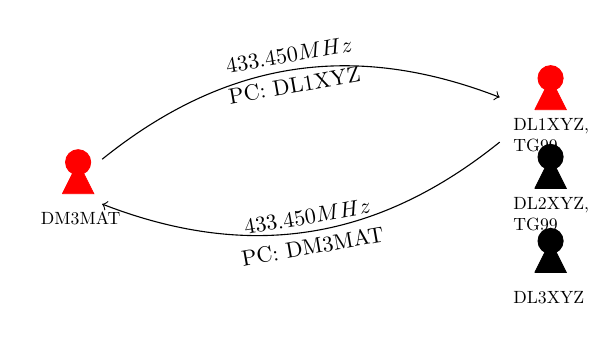
\begin{tikzpicture}[every node/.style={scale=.8}]
  \activeuser{u1}{ 0,0}{DM3MAT};
  \activeuser{u2}{ 6,1}{DL1XYZ, TG99};
  \user{u3}{ 6,0}{DL2XYZ, TG99};
  \user{u4}{ 6,-1}{DL3XYZ};
  \path[->] (u1) edge[bend left] node[above, rotate=10]{$433.450 MHz$} node[below, rotate=10]{PC: DL1XYZ} (u2);
  \path[->] (u2) edge[bend left] node[above, rotate=10]{$433.450 MHz$} node[below, rotate=10]{PC: DM3MAT} (u1);
 \end{tikzpicture}
\end{document}

 \caption{Beispiel eines DMR Simplex Direktrufs von DM3MAT an DL1XYZ.} \label{fig:splxpc}
\end{figure}

In Abbildung \ref{fig:splxpc} ist ein einfache Simplex Direktruf von DM3MAT an DL1XYZ dargestellt sowie die Antwort von DL1XYZ and DM3MAT. Beide senden und empfangen auf der selben Frequenz (hier der DMR Simplex Anruffrequenz von $433.450 MHz$). Auch wenn die beiden anderen Teilnehmer in der Nähe (DL2XYZ \& DL3XYZ) diesen Ruf physisch empfangen, bleiben deren Funkgeräte stumm. Wie dem auch sei, der Kanal ist jedoch während dieses Direktrufes belegt. 

An dieser Stelle ist es sinnvoll zu erwähnen, dass wenn DL1XYZ direkt auf den Direktruf von DM3MAT antwortet indem er die PTT Taste drückt, er mit einem Direktruf an DM3MAT antwortet ohne dafür die Nummer von DM3MAT aus seinen Kontakten heraussuchen zu müssen. Diese Eigenschaft heißt \adef{Talkaround} und funktioniert nur wenige Sekunden nach dem Ende des initialen Direktrufs durch DM3MAT. Nach dieser Zeitspanne wird beim drücken auf die PTT der Standardkontakt für diesen Kanal angerufen, der für jeden Kanal im Funkgerät festgelegt werden kann (siehe Abs. \ref{sec:cp:channel}). Diese Zeitspanne lässt sich auch im Funkgerät einstellen.

\begin{figure}[!ht]
  \centering
  \documentclass{standalone}
\usepackage{tikz}
\usetikzlibrary{shapes.geometric}
\newcommand{\repeater}[3]{%
 \node ({#1}) at ({#2}) {%
  \begin{tikzpicture}%
   \draw [black,thick] (-.25,0) -- (0,0.5) -- (0.25,0) -- (-0.25,0);%
   \draw [black,thick,domain=-45:225] plot ({0.2*cos(\x)}, {0.5+0.2*sin(\x)});%
   \draw [black,thick,domain=-45:225] plot ({0.4*cos(\x)}, {0.5+0.4*sin(\x)});%
   \node (xxx) at (0,-.2) {{#3}};%
  \end{tikzpicture}%
 } %
}

\newcommand{\activerepeater}[3]{%
 \node ({#1}) at ({#2}) {%
  \begin{tikzpicture}%
   \draw [black,thick] (-.25,0) -- (0,0.5) -- (0.25,0) -- (-0.25,0);%
   \draw [red,thick,domain=-45:225] plot ({0.2*cos(\x)}, {0.5+0.2*sin(\x)});%
   \draw [red,thick,domain=-45:225] plot ({0.4*cos(\x)}, {0.5+0.4*sin(\x)});%
   \node (xxx) at (0,-.2) {{#3}};%
  \end{tikzpicture}%
 } %
}


\newcommand{\user}[3]{%
 \node ({#1}) at ({#2}) {%
  \begin{tikzpicture}%
   \draw [black,fill=black] (-.25,0) -- (0,0.5) -- (0.25,0) -- (-0.25,0);%
   \draw [black,fill=black] (0,.5) circle (.2); %
   \node (xxx) [text width=0.6cm, align=center] at (-.35cm,-.4) {{#3}};%
  \end{tikzpicture}%
 } %
}

\newcommand{\activeuser}[3]{%
 \node ({#1}) at ({#2}) {%
  \begin{tikzpicture}%
   \draw [red,fill=red] (-.25,0) -- (0,0.5) -- (0.25,0) -- (-0.25,0);%
   \draw [red,fill=red] (0,.5) circle (.2); %
   \node (xxx) [text width=0.6cm, align=center] at (-.35cm,-.4) {{#3}};%
  \end{tikzpicture}%
 } %
}

\begin{document}
  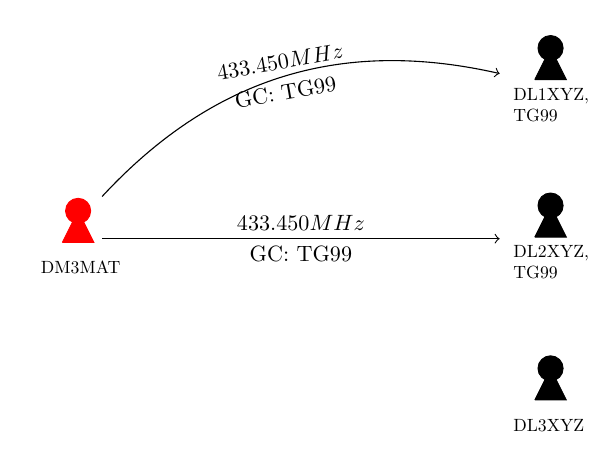
\begin{tikzpicture}[every node/.style={scale=.8}]
   \activeuser{u1}{ 0,0}{DM3MAT};
   \user{u2}{ 6,2}{DL1XYZ, TG99};
   \user{u3}{ 6,0}{DL2XYZ, TG99};
   \user{u4}{ 6,-2}{DL3XYZ};
   \path[->] (u1) edge[bend left] node[above, rotate=10]{$433.450 MHz$} node[below, rotate=10]{GC: TG99} (u2);
   \path[->] (u1) edge node[above]{$433.450 MHz$} node[below]{GC: TG99} (u3);
  \end{tikzpicture}
\end{document}

  \caption{Beispiel eines DMR Simplex Gruppenrufs von DM3MAT an die Sprechgruppe TG99.} \label{fig:splxgc}
\end{figure}

Um im Simplexbetrieb nicht nur einzelne Teilnehmer anrufen zu können, sind auch Gruppenrufe im Simplexbetrieb möglich. Eine beliebte Sprechgruppe (Talk Group) für den Simplex Betrieb ist die Gruppe mit der Nummer 99, daher mit TG99 abgekürzt für \emph{talk group 99}. Solche Gruppenrufe werden dann von allen Funkgeräten empfangen, die entsprechend konfiguriert wurden. Wie beim Repeaterbetrieb muss auch beim Simplexbetrieb dem Funkgerät mitgeteilt werden, welche Sprechgruppen es auf welchen Kanälen empfangen soll (siehe Abs. \ref{sec:cp:rxgrplst}). 

In Abbildung \ref{fig:splxgc} ist solch ein Simplex Gruppenruf von DM3MAT an die Sprechgruppe TG99 dargestellt. Da DL1XYZ und DL2XYZ ihre Funkgeräte so konfiguriert haben, dass sie die TG99 empfangen, hören sie den Ruf von DM3MAT. Da DL3XYZ dies nicht gemacht hat, empfängt er diesen Ruf nicht. DL1XYZ und DL2XYZ können nun auf diesen Gruppenruf antworten, wenn sie innerhalb der sog. \aref{Hangtime} auf ihre PTT Taste drücken. Sie würden dann ebenfalls mit einem Gruppenruf zur TG99 antworten (Talkaround gilt auch für Gruppenrufe), auch wenn sie einen anderen Standardkontakt für diesen Simplexkanal eingestellt haben.

\begin{figure}[!ht]
  \centering
  \input{../fig/simplex_allcall}
  \caption{Beispiel eines DMR All Calls von DM3MAT alle die ihn hören können.} \label{fig:splxac}
\end{figure}

Um wirklich sicher zu gehen, dass ein Ruf auf einem Simplexkanal von allen empfangen werden kann, sollte ein sogenannter \adef{All Call} verwendet werden. Dieser Ruf ist ein spezieller Ruf an eine ganz bestimmte Nummer ($16777215$), die von allen Geräten empfangen werden unabhängig von der Konfiguration dieser Geräte. In diesem Beispiel wird somit der Ruf von DM3MAT auch von DL3XYZ empfangen. Durch \emph{Talkaround} ist es allen Teilnehmern wieder möglich auf den All Call von DM3MAT zu antworten, auch wenn diese Teilnehmer den All Call nicht als den Standardkontakt für diesen Kanal konfiguriert haben. 

\subsection{DMR Simplex Frequenzen}
\begin{table}[!ht]
 \centering
 \begin{tabular}{|l|c||l|c|} \hline
  Name & Frequenz & Name & Frequenz \\ \hline \hline
  S0 (Anruf) & $433.4500 MHz$ & S4 & $433.6500 MHz$ \\
  S1         & $433.6125 MHz$ & S5 & $433.6625 MHz$ \\
  S2         & $433.6250 MHz$ & S6 & $433.6750 MHz$ \\
  S3         & $433.6375 MHz$ & S7 & $433.6875 MHz$ \\ \hline
 \end{tabular}
 \caption{Liste der acht üblichen DMR Simplexkanäle. Der Kanal \emph{S0} ist der Anrufkanal.} \label{tab:simplex}
\end{table}

Im Tabelle \ref{tab:simplex} sind die acht üblichen Simplexkanäle aufgelistet. Der Simplexkanal \emph{S0} ist dabei der Anrufkanal. Gerade in Ballungsgebieten sollte für das eigentliche QSO der Kanal vom Anrufkanal auf einen der sieben weiteren Simplexkanäle \emph{S1-7} gewechselt werden, um den Anrufkanal nicht zu blockieren. 